% !TEX root =  master.tex
\chapter{Database specification}

In the subsequent section, the specifics of the database will be explained. Figure \ref{fig:erd} showcases the Entity-Relationship Diagram (ERD) for the database schema which visually represents the structure of the implemented database. In the following, detailed definitions for used tables, relationships, views and stored procedures will be explained too.

\begin{figure}[htbp]
	\centering
	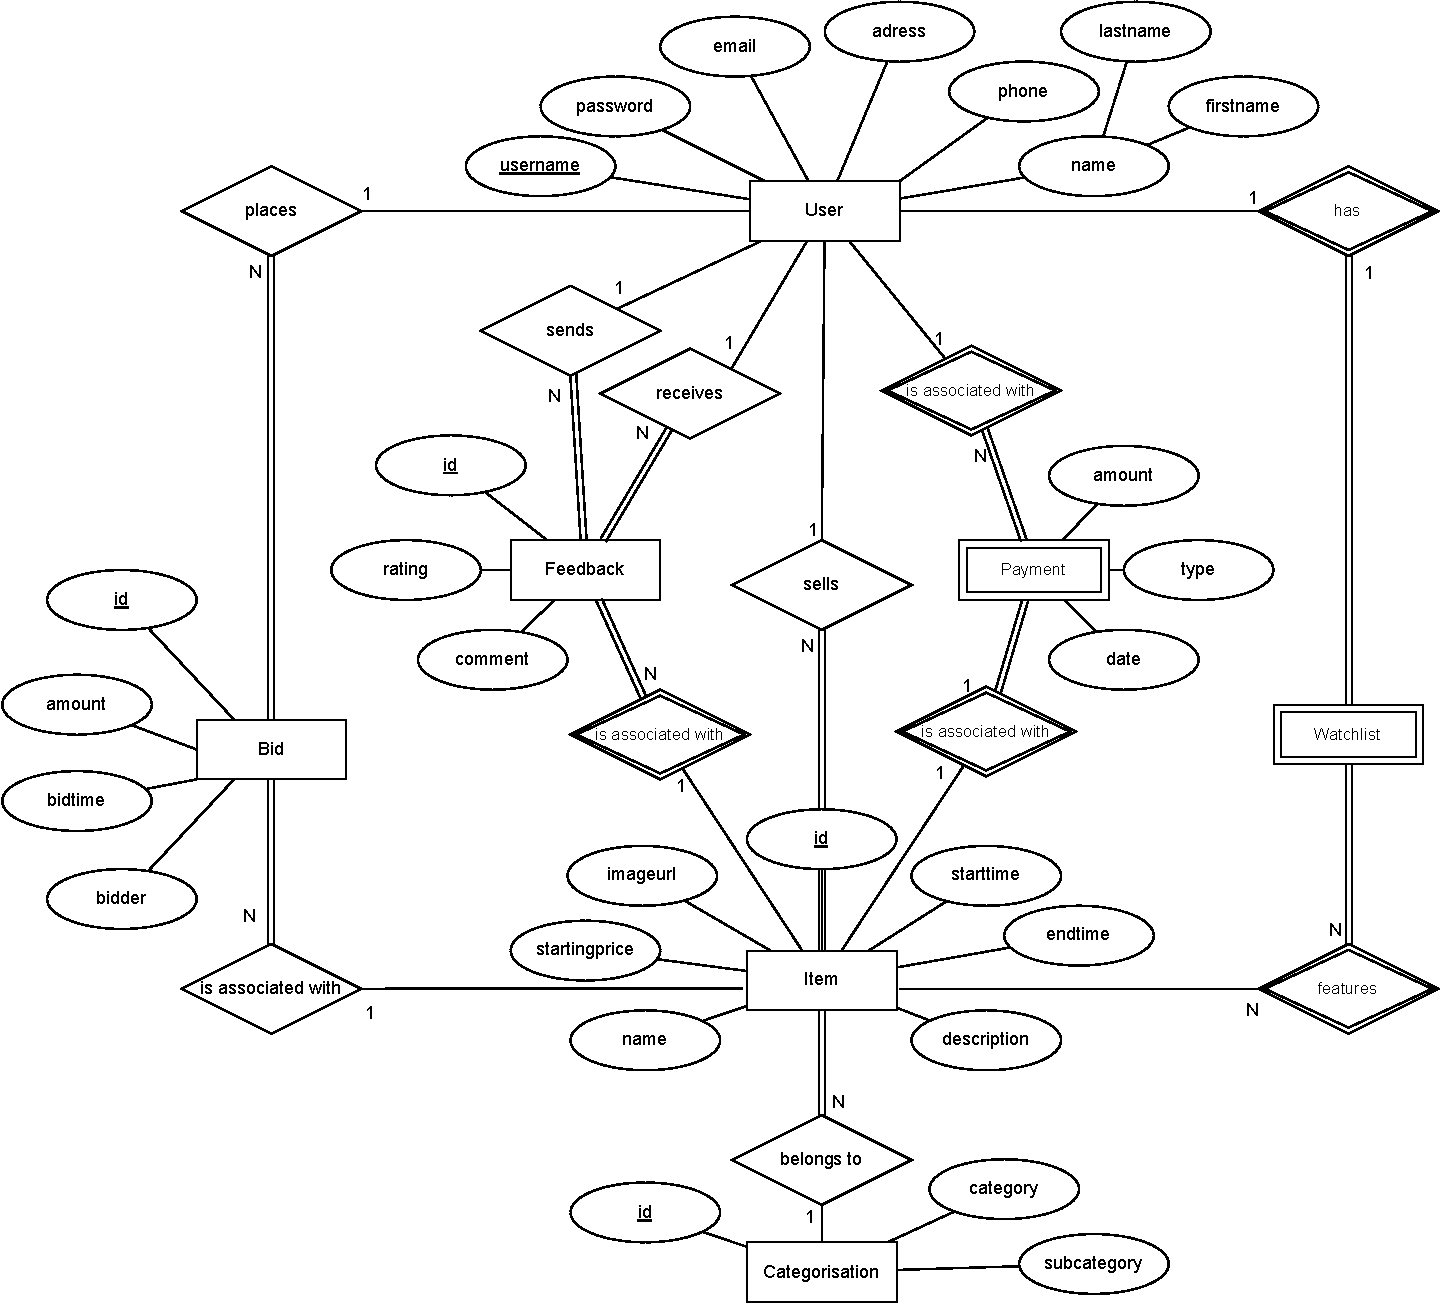
\includegraphics[width=0.7\textheight]{img/ERD-Chen.pdf}
	\caption{Entity-Relationship Diagram}
	\label{fig:erd-chen}
\end{figure}

\section{Tables}

The user table is designed to store all details about the users of the auction system. This includes columns such as 'username', which serves as the primary key and a unique identifier for each user, 'email', the user's unique email address, 'password', the user's hashed password for enhanced security, 'firstName' and 'lastName', which are the first and last name of the user respectively, 'name', a composite of the first and last names, 'address', the user's physical address, and 'phone', the unique phone number of the user. All attributes must have values to create a new user entry.

\begin{lstlisting}[style=sqlStyle]
	CREATE TABLE "user" (
		username VARCHAR(255) PRIMARY KEY,
		email EMAIL NOT NULL UNIQUE,
		password VARCHAR(255) NOT NULL,
		firstName VARCHAR(50) NOT NULL,
		lastName VARCHAR(50) NOT NULL,
		name VARCHAR(100) GENERATED ALWAYS AS (firstName || ' ' || lastName) STORED,
		address TEXT NOT NULL,
		phone VARCHAR(20) NOT NULL UNIQUE
	);
\end{lstlisting}

The item table is responsible for tracking all items listed for auction. It comprises columns such as 'id', a unique identifier for each item and the primary key for this table, 'name', the item's name, 'description', a detailed description of the item, 'startingPrice', the initial price for the auction of this item, 'startTime' and 'endTime', the timestamps for the beginning and end of the auction, 'imageUrl', the URL for an image of the item, 'user\_username', the username of the user who listed the item, a foreign key referencing the user table, and 'category\_id', the id of the item's category, a foreign key referencing the categorisation table.

\begin{lstlisting}[style=sqlStyle]
	CREATE TABLE Item (
		id INTEGER DEFAULT nextval('item_sequence') PRIMARY KEY,
		name VARCHAR(50) NOT NULL,
		description TEXT NOT NULL,
		startingPrice NUMERIC DEFAULT 0,
		startTime TIMESTAMP NOT NULL,
		endTime TIMESTAMP NOT NULL,
		imageUrl TEXT NOT NULL,
		user_username VARCHAR(50) REFERENCES "user"(username)
	ON DELETE SET NULL,
		category_id INTEGER REFERENCES Categorisation(id)
	);
\end{lstlisting}

The categorisation table categorizes the items being auctioned. It consists of three columns - 'id', 'category', and 'subcategory'. 'id' is a unique identifier for each category or subcategory pairing and serves as the primary key for this table. 'category' and 'subcategory' are text-based columns that describe the item category and the corresponding subcategory.

\begin{lstlisting}[style=sqlStyle]
	CREATE TABLE Categorisation (
		id SERIAL PRIMARY KEY,
		category VARCHAR(50) NOT NULL,
		subcategory VARCHAR(50) NOT NULL
	);
\end{lstlisting}

The bid table contains information regarding all bids placed on the items. It includes 'id', a unique identifier for each bid and the primary key for this table, 'amount', the bid's amount, 'bidTime', the timestamp when the bid was placed, 'user\_username', the username of the user who placed the bid, a foreign key referencing the user table, and 'item\_id', the id of the item being bid on, a foreign key referencing the item table.

\begin{lstlisting}[style=sqlStyle]
	CREATE TABLE Bid (
		id SERIAL PRIMARY KEY,
		amount NUMERIC NOT NULL,
		bidTime TIMESTAMP NOT NULL,
		user_username VARCHAR(50) REFERENCES "user"(username)
	ON DELETE SET NULL,
		item_id INTEGER REFERENCES Item(id)
	);
\end{lstlisting}

The watchlist table allows users to track items they are interested in. It includes 'user\_username', the username of the user interested in an item, a foreign key referencing the user table, and 'item\_id', the id of the item the user is interested in, a foreign key referencing the item table. The combination of 'user\_username' and 'item\_id' is unique, preventing duplicate entries in the watchlist.

\begin{lstlisting}[style=sqlStyle]
	CREATE TABLE Watchlist (
		user_username VARCHAR(50) REFERENCES "user"(username)
	ON DELETE CASCADE,
		item_id SERIAL REFERENCES Item(id),
	CONSTRAINT unique_watchlist_entry UNIQUE (user_username, item_id)
	);
\end{lstlisting}

The feedback table facilitates users in leaving feedback about their transactions. It comprises 'feedbackID', a unique identifier for each feedback and the primary key for this table, 'item-id', the id of the item which was sold and to which the feedback is refering, 'rating', the rating given by the sender to the receiver on a scale from 0 to 10, 'comment', a text field for additional comments, 'sender' and 'receiver', the usernames of the user giving and receiving the feedback, both foreign keys referencing the user table.

\begin{lstlisting}[style=sqlStyle]
	CREATE TABLE Feedback (
		feedbackID SERIAL PRIMARY KEY,
		item_id INTEGER REFERENCES Item(id),
		rating INTEGER NOT NULL CHECK (rating BETWEEN 0 AND 10),
		comment TEXT,
		sender VARCHAR(50) REFERENCES "user"(username)
	ON DELETE SET NULL,
		receiver VARCHAR(50) REFERENCES "user"(username)
	ON DELETE SET NULL
	);
\end{lstlisting}

The payment table records all payments made for the items. It includes 'amount', the amount paid, 'date', the timestamp when the payment was made, 'type', the method of payment, 'user\_username', the username of the user making the payment, a foreign key referencing the user table, and 'item\_id', the id of the item for which the payment was made, a foreign key referencing the item table.

\begin{lstlisting}[style=sqlStyle]
	CREATE TABLE Payment (
		amount NUMERIC NOT NULL,
		date TIMESTAMP NOT NULL,
		type PAYMENT_TYPE NOT NULL,
		user_username VARCHAR(50) REFERENCES "user"(username)
	ON DELETE SET NULL,
		item_id INTEGER REFERENCES Item(id)
	);
\end{lstlisting}


\section{Relationships}
\textbf{User Table - Item Table}: Each user can list many items for auction, but each item is listed by only one user. The relationship is established via the user\_username foreign key in the Item table.

\textbf{User Table - Bid Table}: Each user can place many bids, but each bid is placed by only one user. This relationship is established via the user\_username foreign key in the Bid table.

\textbf{User Table - Watchlist Table}: Each user can have many items on their watchlist, but each watchlist entry is linked to only one user. This relationship is established via the user\_username foreign key in the Watchlist table.

\textbf{User Table - Feedback Table}: Each user can both give and receive feedback many times, but each feedback entry is given by and given to only one user. This relationship is established via the sender and receiver foreign keys in the Feedback table.

\textbf{User Table - Payment Table}: Each user can make many payments, but each payment is made by only one user. This relationship is established via the user\_username foreign key in the Payment table.

\textbf{Item Table - Bid Table}: Each item can have many bids, but each bid is placed on only one item. The relationship is established via the item\_id foreign key in the Bid table.

\textbf{Item Table - Watchlist Table}: Each item can be on the watchlist of many users, but each watchlist entry is for only one item. This relationship is established via the item\_id foreign key in the Watchlist table.

\textbf{Item Table - Payment Table}: Each item has one payment associated with it, and each payment is linked to only one item. This relationship is established via the item\_id foreign key in the Payment table.

\textbf{Categorisation Table - Item Table}: Each category can have many items, but each item belongs to only one category. The relationship is established through the category\_id foreign key in the Item table.


\section{Views}
The database also consists of two views, item\_status and user\_statistics.
The items\_status view is created to show the current status of each item in the auction. It contains various fields that provide important information about the item, its current highest bid, and the related users (highest bidder and seller). The purpose of this view is to aggregate relevant data from multiple tables and present it in a more readable and understandable format. It can be used to display the current state of items in a user-friendly way on an application or website.

The view is created by joining the item table with a subquery that calculates the highest bid for each item. The result is then joined with the bid table to retrieve the highest bidder's username. The selected fields in this view include the item's name, id, description, image URL, remaining time until the auction ends, the highest bid, the highest bidder's username, and the seller's username.
\begin{lstlisting}[style=sqlStyle]
	CREATE VIEW items_status AS
	SELECT 
		item.name AS title, 
		item.id AS item_id, 
		item.description, 
		item.imageUrl AS image_path,  
		EXTRACT(DAY FROM AGE(item.endtime, CURRENT_TIMESTAMP)) AS time_left,
		max_bids.highest_bid,
		bid.user_username AS highest_bidder,
		item.user_username AS seller
	FROM item 
	JOIN (SELECT item_id, MAX(amount) AS highest_bid FROM bid GROUP BY item_id) AS max_bids 
	ON item.id = max_bids.item_id
	JOIN bid
	ON bid.item_id = max_bids.item_id
	AND bid.amount = max_bids.highest_bid;
\end{lstlisting}

The user\_statistics materialized view in the database provides an aggregated summary of user activities on the auction platform. Being a materialized view, it stores the result of a complex and potentially time-consuming query, which can be refreshed as required, leading to faster data retrieval.

Each row in this view represents a unique user on the platform. The view contains a variety of fields calculated from different tables to give a comprehensive overview of each user's auction activities. The participated\_auctions field shows the total number of unique auctions where the user has placed a bid, as determined from the bid table. Another field, won\_auctions, displays the number of auctions that the user has won. It's calculated from the bid table, where the user's bid was the highest and the auction time had ended. The average\_rating field indicates the mean feedback rating received by the user. It's derived from the feedback table by averaging all the ratings received by a user.
To understand the financial aspect, two more fields are included: total\_expenses and total\_income. total\_expenses shows the sum of all the payments made by a user for won auctions, calculated from the payment table. On the other hand, total\_income calculates the total amount received by a user for the items they have sold. It's calculated by joining the payment and item tables and summing up the amounts where the user is the seller.

\begin{lstlisting}[style=sqlStyle]
	CREATE MATERIALIZED VIEW user_statistics AS
	SELECT 
		u.username,
		COALESCE(participated_auctions.participated_auctions, 0) AS participated_auctions,
		COALESCE(won_auctions.won_auctions, 0) AS won_auctions,
		COALESCE(CAST(average_feedback.average_rating AS INTEGER), 0) AS average_rating,
		COALESCE(total_expenses.total_expenses, 0) AS total_expenses,
		COALESCE(total_income.total_income, 0) AS total_income
	FROM "user" u
	LEFT JOIN (
	SELECT user_username, COUNT(DISTINCT item_id) AS participated_auctions
	FROM bid
	GROUP BY user_username
	) AS participated_auctions ON u.username = participated_auctions.user_username
	LEFT JOIN (
	SELECT user_username, COUNT(DISTINCT bid.item_id) AS won_auctions
	FROM bid
	JOIN items_status ON bid.item_id = items_status.item_id AND bid.amount = items_status.highest_bid
	WHERE items_status.time_left < 0
	GROUP BY user_username
	) AS won_auctions ON u.username = won_auctions.user_username
	LEFT JOIN (
	SELECT receiver, AVG(rating) AS average_rating
	FROM feedback
	GROUP BY receiver
	) AS average_feedback ON u.username = average_feedback.receiver
	LEFT JOIN (
	SELECT user_username AS buyer, SUM(amount) AS total_expenses
	FROM payment
	GROUP BY user_username
	) AS total_expenses ON u.username = total_expenses.buyer
	LEFT JOIN (
	SELECT item.user_username AS seller, SUM(amount) AS total_income
	FROM payment
	JOIN item ON item.id = payment.item_id
	GROUP BY item.user_username
	) AS total_income ON u.username = total_income.seller;
\end{lstlisting}


\section{Stored Procedure}
The purpose of the implemented stored procedure is to add a random item to the watchlist of a user when the user account is created. The item must be currently on auction, meaning its end time must be in the future.

A variable random\_item\_id of type integer is declared to store the id of a randomly selected item. It executes a SELECT query to get the id of a random item that is currently on auction. This is done by ordering the items from the items\_status view (which contains the items with their current status) randomly and selecting the first one. Once it has the id of a random item, it inserts a new row into the watchlist table with the username of the new user and the id of the randomly selected item.

This stored procedure is run by a trigger named user\_created\_trigger. A trigger is a special type of stored procedure that runs automatically when an event associated with a table occurs such as insert, update, or delete. In this case, the trigger is configured to run the add\_random\_item\_to\_watchlist() stored procedure each time a new row is inserted into the user table. This is specified by the AFTER INSERT ON "user" part of the trigger creation statement.

\begin{lstlisting}[style=sqlStyle]
	CREATE OR REPLACE FUNCTION add_random_item_to_watchlist()
	RETURNS TRIGGER AS $$
	DECLARE
		random_item_id INTEGER;
	BEGIN
	
	-- Get the id of a random item which is currently on auction
	SELECT item_id
	FROM items_status
	WHERE time_left > 0
	ORDER BY RANDOM()
	LIMIT 1
	INTO random_item_id;
	
	-- Put that item on the watchlist of the newly created user
	INSERT INTO watchlist (user_username, item_id)
	VALUES (NEW.username, random_item_id);
	
	RETURN NEW;
	END;
	
	$$ LANGUAGE plpgsql;
	
	-- Create a trigger that executes the stored procedure whenever a new entry is added to the user table
	CREATE TRIGGER user_created_trigger
	AFTER INSERT ON "user"
	FOR EACH ROW
	EXECUTE FUNCTION add_random_item_to_watchlist();
\end{lstlisting}
